\documentclass{article}
\usepackage{graphicx}

\begin{document}

\title{Team Meeting 1 Summary}
\author{Christian Plourde 26572499\\*
		Ayush Kharade 40042388\\*
		Daniel Vellucci 27416288\\*
		Samer Yazbeck 40049573\\*
		Luciano Porchet 40048537
		}
\date{September 18th, 2019}

\maketitle

\newpage

\section{Meeting Duration}
75 Minutes

\section{Notes}
\subsection{Game Details}
\begin{description}
\item 3D characters, Platformer in a 2D view
\item Platformer
\item Singleplayer
\item Similar to Trine or This War of Mine
\item Genre: Action / Adventure platformer
\end{description}

\subsection{Story}
\begin{description}
\item Starts with “Hey you're finally awake!”\\*(wake up in a cave? Forest?, need a setting)
\item The Lord Ruler is dead, Ruin has been released.
\item Ruin is trying to destroy the world and has gained control of minions and people who become the enemies
\item Main character is fighting for survival and ends up destroying ruin in the end (or a higher level minion control directly by Ruin), so ruin is still out there, the possibility for a sequel.
\item Main character doesn't want to save the world but gets forced into doing it (joke story) 
\end{description}

\subsection{Enemies}
\begin{description}
\item Mistings (people who can burn one metal)
\item Koloss (large enemies that wield swords)
\item Coinshots(ranged?)
\item Regular minions (people under Ruin’s Control)
\end{description}

\subsection{Mistborn Mechanics}
\begin{description}
\item Burning metals (magic system called allomancy)
\item Iron - pull metal objects toward you
\item Steel - push metal objects away from you
\item Brass - Sooth people's emotions (could be used to make people fall asleep) (throwable?)
\item Zinc - Riot people's emotions (could be used to charm enemies to fight for you) (throwable?)
\item Tin - Heightens senses (could be used to see enemies past the fog of war)
\item Pewter - Makes user stronger, more agile, increases endurance and healing
\item Bronze - Detect another person burning metals (made from copper and tin)
\item Copper - Hide your metal burning from other people
\item Gold - See yourself in the past (is it implementable?)
\item Atium - see another person a few moments in the future (is it implementable?)
\item Collect metals from the environment
\item Hidden metals, scavenging
\item Crafted metals
\item Progression in usability of metal (start with a few, unlock more as you progress)
\item NPC to provide metals for you (buyable from shops)
\item Combining metals for different effects? (Could have it so you can't get steel without combining iron and carbon) (or iron and carbon do two different things but when combined they make objects static, this could be used for stasis puzzle mechanics)
\item Fog of war idea (light coming from player), only things that are illuminated can be affected by allomancy, or faint light coming from every character
\item Small puzzles to find rare metals
\item Ruin can change words (give fake hints to the player) player gambles if it is worth going there (could have traps or very powerful enemies in these areas)
\item Collect carbon from everywhere, if you don't use it all game it turns into diamond and you get an ultimate ability
\end{description}

\subsection{Combining Metals Mechanic}
\begin{description}
\item Alchemy table to combine metals or unlockable \& portable mortar and pestle (need to be out of combat or at a save point to combine metals)
\item Skill tree could be accessed from here too (requires to unlock skill to combine metals)
\end{description}

\subsection{Mistborn Setting}
\begin{description}
\item Black world, falling ash, red sun
\item Misty Environment
\item Mistcloaks
\end{description}

\subsection{Combat}
\begin{description}
\item Steel, iron fighting moving metal objects
\item Melee only available when you burn pewter
\end{description}

\subsection{Enemy Mechanics}
\begin{description}
\item Only attack if close enough, move towards you until it is close enough
\item Chase you to the end of the room then go back
\end{description}

\subsection{Supporting Art}
  \begin{figure}[!htb]
    \center{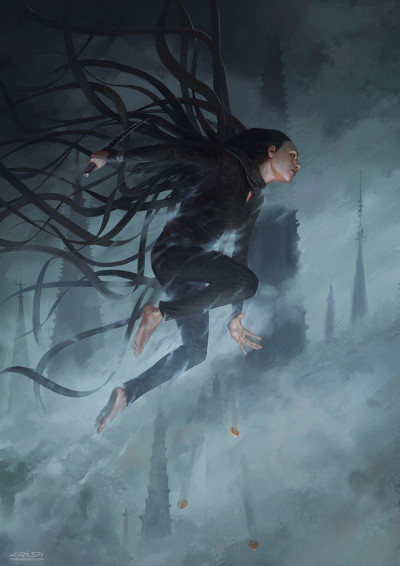
\includegraphics[width=\textwidth]
    {vin_1.png}}
  \end{figure}

  \begin{figure}[!htb]
    \center{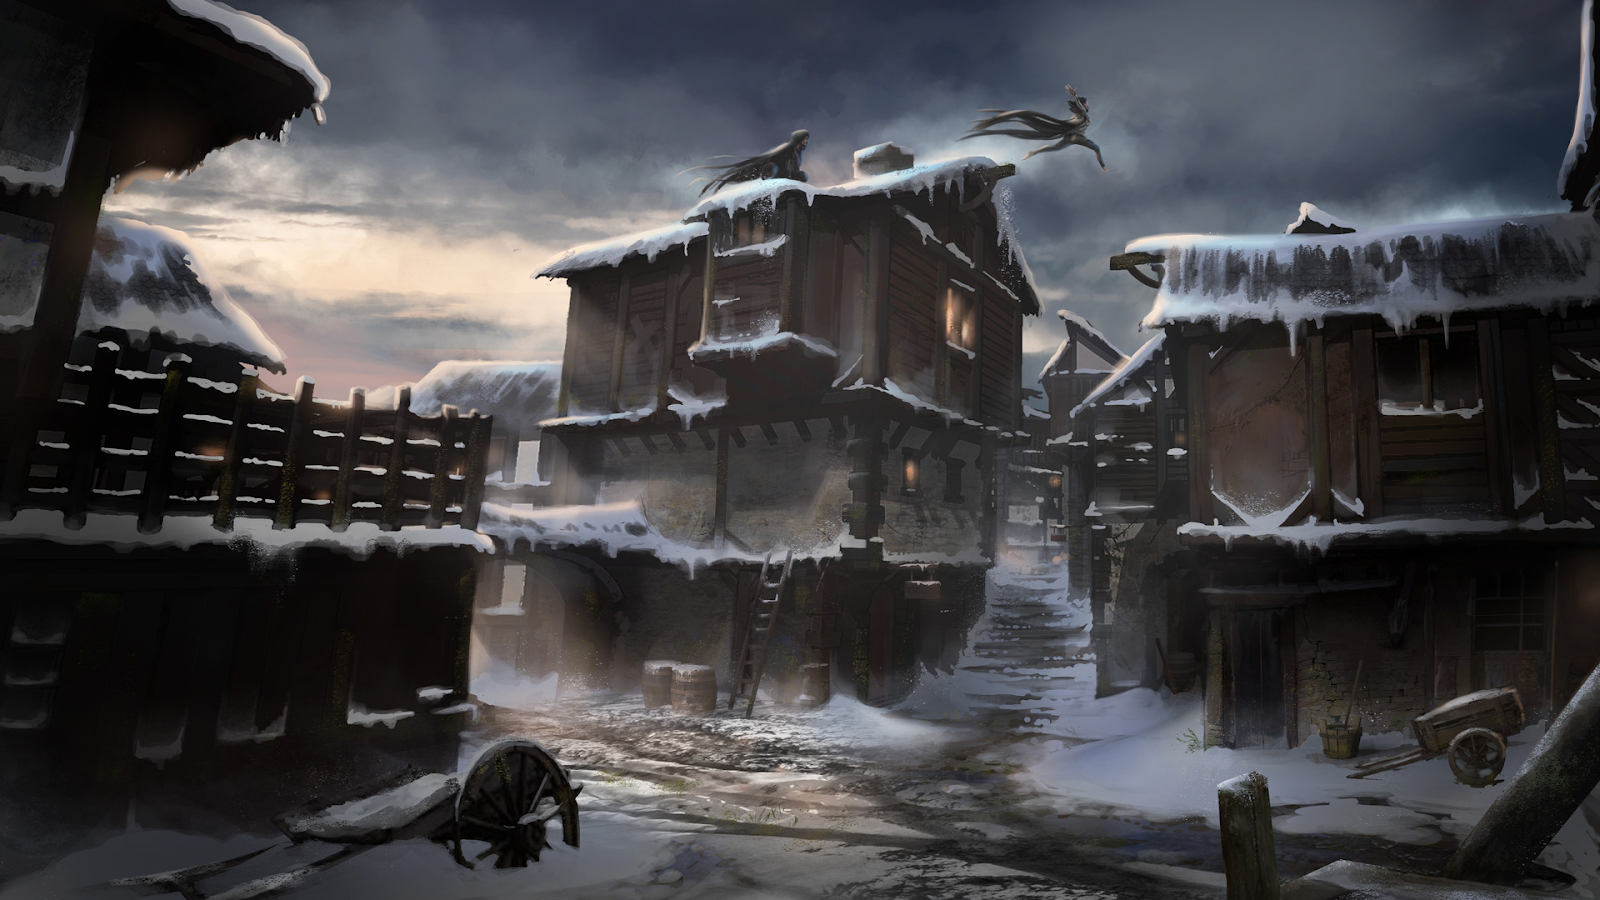
\includegraphics[width=\textwidth]
    {luthadel_0.png}}
  \end{figure}

  \begin{figure}[!htb]
    \center{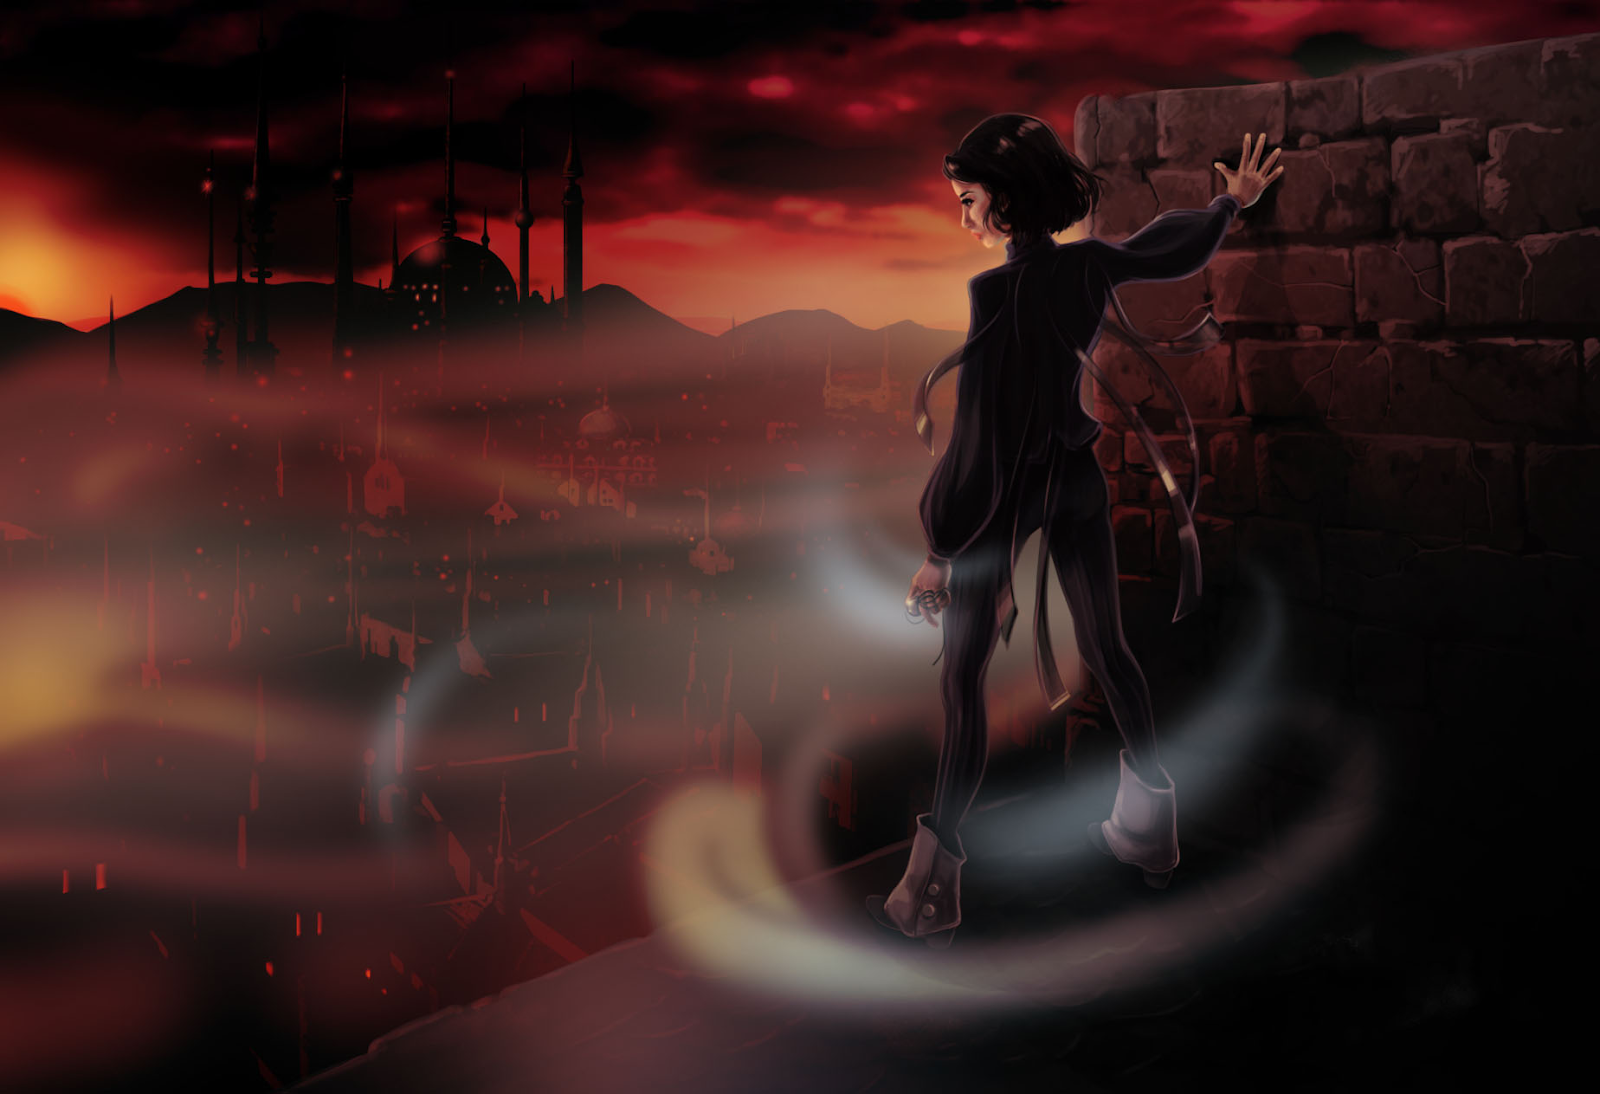
\includegraphics[width=\textwidth]
    {luthadel_1.png}}
  \end{figure}
\end{document}